%\chapter[<ToC-title>]{<Title>} 
\chapter[\DataStrToCTitle]{\DataStrTitle}
\label{chap:DataStr}

Detecting correspondences between different spatial datasets
has been drawn a lot of attention in map generalization 
\parencite[e.g.,][]{Noellenburg2008,Peng2016Admin,Deng2015}
and data conflation 
\parencite[e.g.,][]{Zhang2008Matching,Masuyama2006Tessellation,
	Tong2014Matching,Ruiz2011Conflation}.
A reason is that corresponding objects,
which represent the same real-world entity,
may have different coordinates; 
measurements introduce errors, 
and different organizations may use their own approaches 
to produce datasets \parencite{Beeri2005}.
An important criteria of determining corresponding objects
is to investigate if they have close positions. 
For example, \textcite{Beeri2005} assumed that 
the locations of objects are given as points 
and required that corresponding objects should have a distance 
smaller than a threshold.
Based on the work of \textcite{Beeri2005}, 
\textcite{Safra2013} managed to match road networks.
\textcite{Volz2006} matched street data 
starting from so-called \emph{seed nodes}.
Each pair of their seed nodes should be 
within a distance of~$30\,$meters.
We model the problem of looking for 
\emph{close} points as follows.
For a given set of points,
we want to find all the pairs of close points. 
We consider two points to be close 
if they lie within a square of a pre-specified 
side length, say,~$\varepsilon$. 
In other words, points~$p$ and~$q$ are close 
if distance~$L_{\infty }(p,q)=\max (\Delta x,\Delta y)
\le \varepsilon$, where 
$\Delta x=\vert p_{x}-q_{x}\vert $ and 
$\Delta y=\vert p_{y}-q_{y}\vert$
are the differences of $x$- and $y$-coordinates, respectively;
see \fig\ref{fig:DataStr_Problem}.

\begin{figure}[tb]
\centering
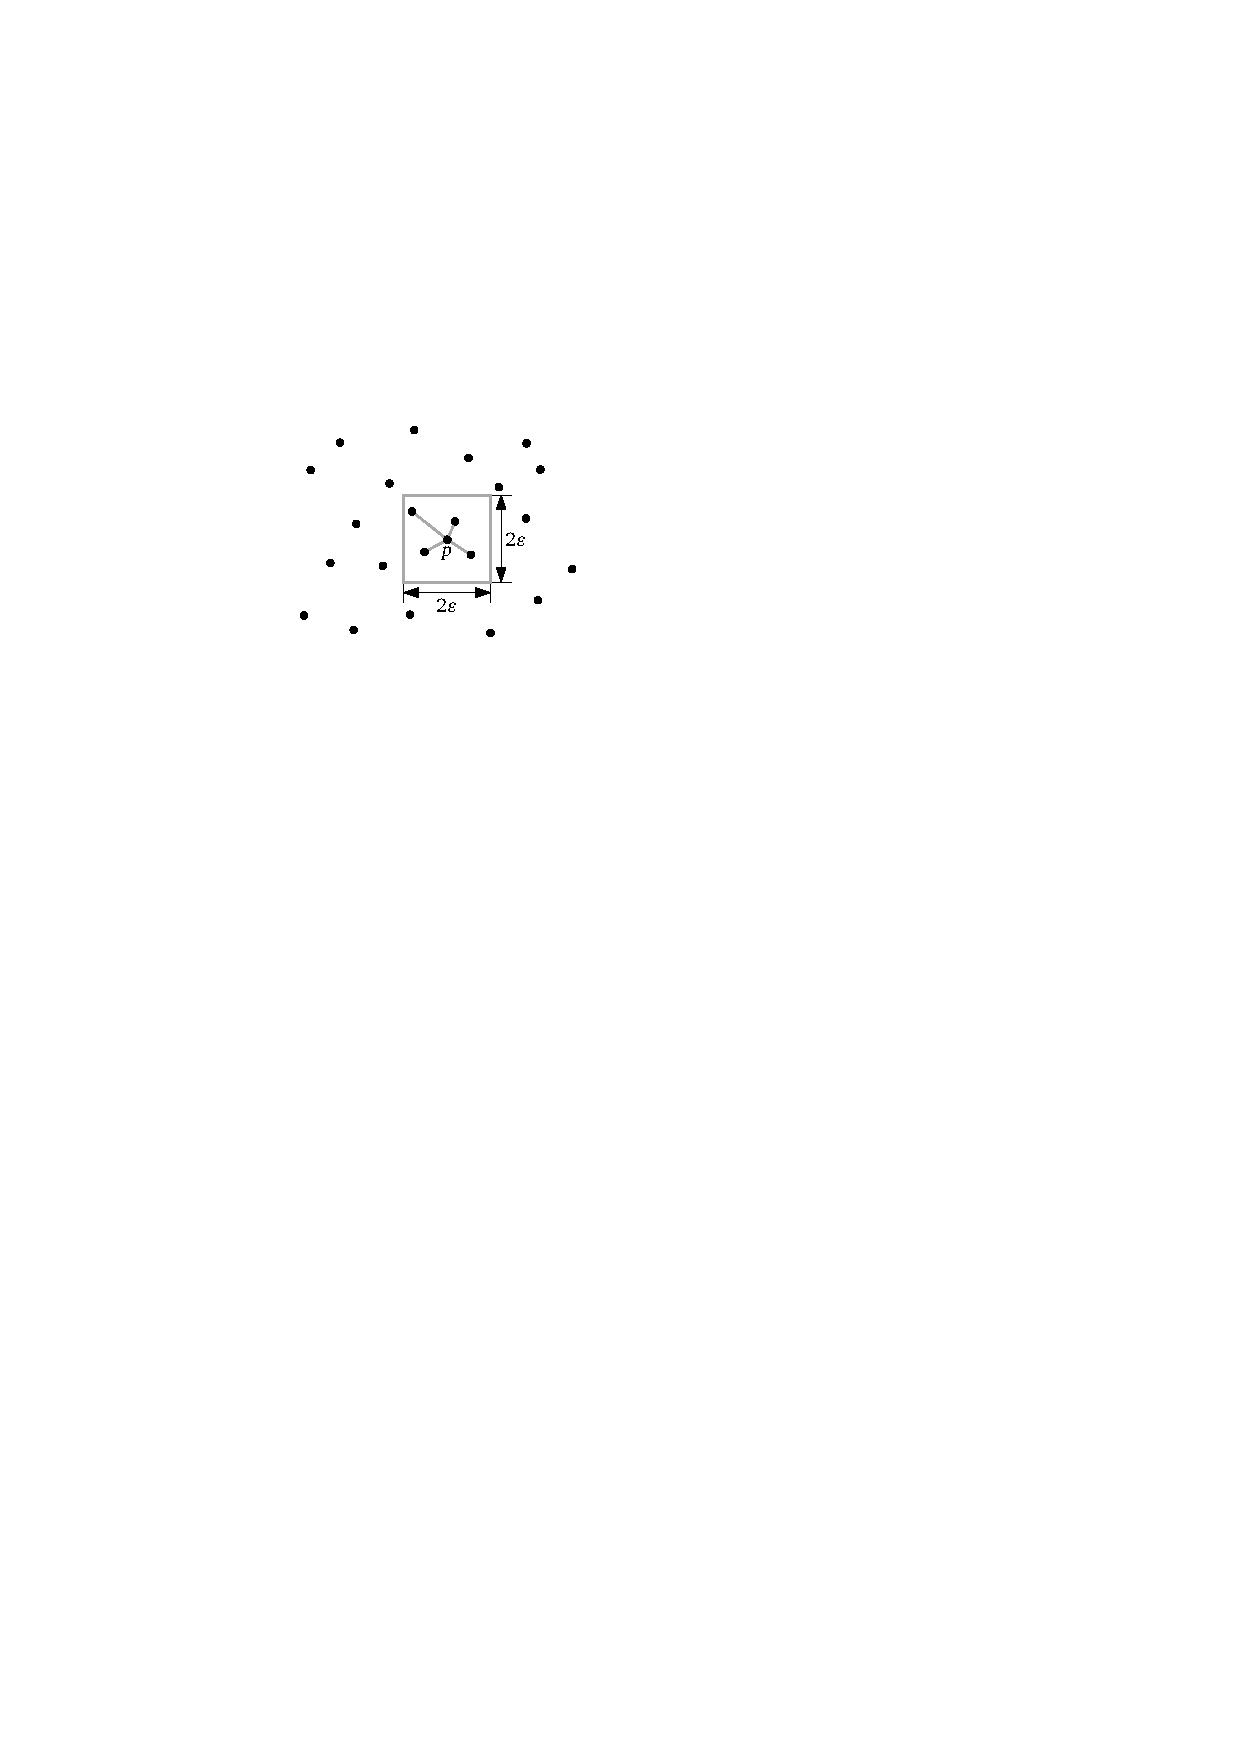
\includegraphics{DataStr_Problem}
\caption{For point~$p$, the four linked points are 
	its close points.
	These close points lie in the square 
	with side length~$2 \varepsilon$ centered at $p$.}
\label{fig:DataStr_Problem}
\end{figure}

When implementing and testing some ad-hoc solutions 
for this problem, 
we made a number of observations 
that we found worth sharing with the GIS community. 
That is to sat, the ultimate goal of this chapter 
is not to identify the algorithm 
that performs best for the problem at hand. 
Instead, we want to address the issues 
that we had during implementing and testing; 
we want to discuss the lessons we learned.


A brute-force approach for finding all pairs of close points 
requires~$\Theta (n^{2})$ time, 
where~$n$ is the number of points. 
This running time is worst-case optimal 
since the size of the output can be~$\Theta (n^{2})$ 
if~$\varepsilon$ is sufficiently large. 
Typically, however, the size of the output is small. 
Hence, it is desirable to use algorithms 
whose running time do not only depend on 
the size of the input ($n$, the number of points), 
but also on the size of the output, that is, 
the number of pairs of close points, 
which we denote by~$k$. 
Such an algorithm is called \emph{output-sensitive}. 
Our problem is different from \textcite{Saalfeld1988}. 
For a given point on one map, they found the 
single nearest point in another map,
which can be accomplished in~$O(n\log n)$ time 
\parencite{Shamos1975}.

We consider three obvious output-sensitive algorithms: 
A sweep-line (SL) algorithm, 
an algorithm based on the Delaunay Triangulation (DT), and 
a hashing-like approach that uses a grid. 
The SL algorithm runs in~$O(k+n\log n)$ worst-case time.
The same running time holds for the DT-based algorithm 
under the assumption that 
the input points are randomly and independently drawn 
in a unit square (see \sect\ref{sec:DataStr_Algorithms}). 
Under the same assumption 
regarding the distribution of the input, 
the grid-based algorithm runs in~$O(k+n)$ time. 
We sketch the three algorithms in 
\sect\ref{sec:DataStr_Algorithms}. 
We have implemented them, and 
we have compared their performances on random data 
and real-world data (see \sect\ref{sec:DataStr_CaseStudy}). 
We conclude the chapter in \sect\ref{sec:DataStr_Conclusion}.



We remark that we focus on methods 
that can be implemented easily.
For this reason we have not included a method that uses 
two-dimensional range trees
\parencite{Bentley1977Multivariate,Lueker1978,Lee1980Tree}, 
which is a two-level data structure based on
balanced binary search tree (BBST);
see \textcite[\chap13]{Cormen2009}.
The method works as follows. 
We insert all~$n$ input points into the range tree 
and then query the tree, for each point~$p$, 
with a range of size~$2\varepsilon \times 2\varepsilon$ 
centered at~$p$.
The running time of this method is~$O(k+n\log ^{2}n)$, the 
memory consumption is~$O(n\log n)$;
see \textcite{Bentley1977Multivariate,}. 
The running time can be improved to~$O(k+n\log n)$ 
by using fractional cascading
\parencite[\chap5]{deBerg2008}, 
but we would need additional implementation effort.





\section{Algorithms}
\label{sec:DataStr_Algorithms}

In the following, we sketch the three algorithms. 
We denote the set of input points 
by~$P=\{p_{1},p_{2},\ldots , p_{n}\}$,
where point~$p_{i}$ has coordinates~$(x_{i},y_{i})$. 
While the algorithms work for any input, 
our running-time analyses will assume 
that the input points are 
uniformly and independently distributed (u.i.d.) 
in the unit square~$[0,1]\times [0,1]$. 
We do not record the pairs of close points 
but just count them, 
thus we need little extra memory for recording the output.



\subsection{The Sweep-Line Algorithm}
\label{sec:DataStr_SLAlgorithm}



The SL paradigm is a common tool in computational geometry
\parencite[\chap2]{deBerg2008}.
\textcite{Shamos1976} developed this algorithm to determine
if two polygons intersect.
In their case, the SL algorithm runs in~$O(n'\log n')$ time,
where~$n'$ is the total number of the edges of the polygons.
\textcite{Bentley1979} extended the SL algorithm so that 
they could report all the intersections.
This extension increases the running time 
to~$O(k' +n'\log n')$,
where $k'$ is the number of intersections. 
Intuitively, the SL algorithm uses a line to sweep the plane, 
then the line stops at certain events 
and changes its internal status
(see \fig\ref{fig:DataStr_SL}).
The SL algorithm usually employs two data structures: 
the \emph{event queue} and the \emph{status}. 
For our problem of searching for close points, 
we sweep a horizontal line from top to bottom. 
Our sweep line~$l: y=y_{l}$ stops at the $y$-coordinates 
in set~$\{ y_{i}, y_{i}-\varepsilon | i=1, 2, \ldots , n\}$.
We store these coordinates
(together with references to the corresponding points) 
in the event queue in decreasing order. 
The status contains all points in a 
horizontal strip of height $ \varepsilon$ 
bounded by lines~$l$ 
and~$l_{\varepsilon}: y=y_{l}+\varepsilon$. 
We store the points according to 
their $x$-coordinates using a BBST in increasing order. 
To implement the event queue, 
it suffices to sort the $2n$ $y-$coordinates 
and store the sorted coordinates in an array.

\begin{figure}[tb]
\centering
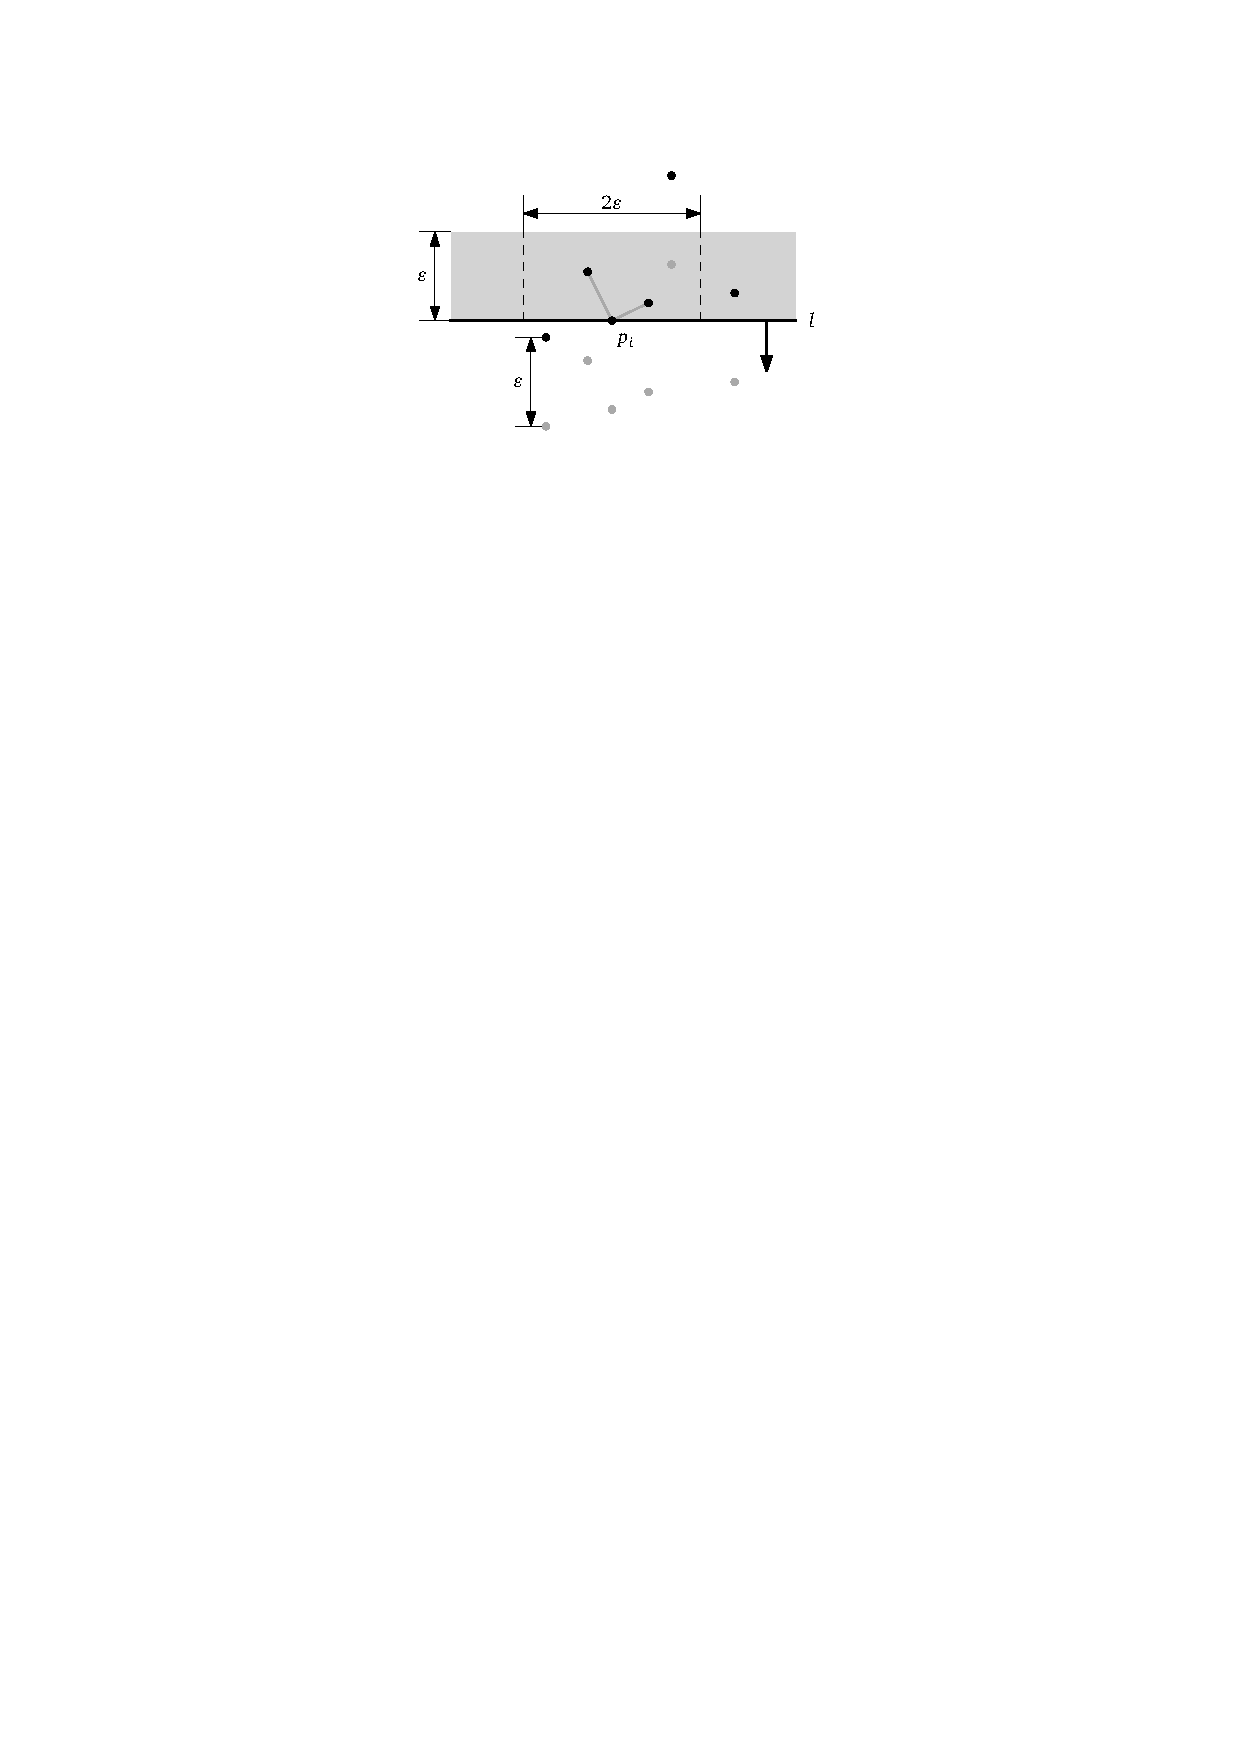
\includegraphics[page=1]{DataStr_Algorithms}
\caption{An illustration of our SL algorithm.
	The sweep line $l$ is moving from top to bottom.
	The black points are the data that 
	we are looking for close points.
	The gray points are the references 
	to the corresponding black points.
	The gray strip represents the status which is 
	implemented by a BBST.
	The black points in the status are 
    the potential close points.
	When the sweep line hits a black point,
	we search for close points in the status and then
	enter the black point into the status;
	when the sweep line hits a gray point, 
	we remove the corresponding black point from the status.
	In this example, the sweep line hits point~$p_i=(x_i, y_i)$. 
	It is sufficient to search in the interval
	$[x_i-\varepsilon, x_i+\varepsilon]$ of the status.
	As a result, we find two close points, 
	which are linked to~$p_i$.
}
\label{fig:DataStr_SL}
\end{figure}

We have only two types of events: \emph{enter} and \emph{leave}.
Point~$p_{i} $ enters the status when the sweep line hits 
it, that is, when $y_{l}=y_{i}$. 
At the same time, we report each pair~$(p_{i},p_{j})$, where 
$p_{j}$ is a point in the status 
with~$x_{i}-\varepsilon \le x_{j}\le x_{i}+\varepsilon$. 
Such a \emph{points-in-interval} query is supported by BBSTs. 
The query takes~$O(k_{i}+\log n)$ time, 
where~$k_{i}$ is the number of points 
that are reported for~$p_{i}$.
Point~$p_{i}$ leaves the status 
when the sweep line reaches the~$y$-coordinate 
$y_{i}-\varepsilon$.
Summing up the running time for each point
yields a total running time of~$O(k+n\log n)$, 
where~$k$ is the size of the output, 
that is, the number of close-point pairs. 
The memory consumption of the SL algorithm is~$O(n)$.

The C\# implementation of BBST is \emph{SortedDictionary} (SD),
which does not offer a specific points-in-interval query. 
Instead, SD offers method \emph{where}, 
which takes an arbitrary predicate as argument 
and returns all currently stored objects 
that fulfill the predicate, but this method takes linear time. 
The linear time is not a problem 
as long as side length~$\varepsilon$ is so small 
that the strip, with height~$\varepsilon$ and above the sweep line, 
never contains many points. 
In the worst case, however, 
the running time becomes quadratic even 
if there is no pair of close points at all. 
Luckily, the BBST implementations 
\emph{SortedSet} (SS) from .NET Framework 4.0 and
\emph{TreeSet} (TS) from library C5
both support the points-in-interval query.
Library C5 is an open-source C\# data structure
from \textcite{Kokholm2006}.
In addition, \emph{TreeSet} of language Java 
also supports the points-in-interval query.



\subsection{The Delaunay-Triangulation-Based Algorithm}
\label{sec:DataStr_DTAlgorithm} 

The DT is a useful tool for partitioning the plane 
such that spatially close points are connected
by the edges of the DT. 
For example, it is well-known that
the line segment between any point and its closest neighbor
is an edge of the DT.
Given the DT, we go through the points 
and start a modified \emph{breadth-first search} (BFS) 
from each of them
\parencite[e.g.,][]{Maus2010AllCN,Rahmati2013}. 
BFS is a well-known graph traversal algorithm
\parencite[chapter 22]{Cormen2009}. 
For input point~$p$, 
our BFS considers every point~$q\ne p$ 
with~$L_{\infty}(p,q)\le (1+\sqrt{2})\varepsilon /2$. 
We say that~$r_{1}=(1+\sqrt{2})\varepsilon /2\approx 
1.2\varepsilon$ 
is the \emph{radius} of our BFS. 
The reason for using~$r_{1} $ is simply that 
a radius of~$\varepsilon$ is not sufficient; 
we may, in rare cases, oversee some pairs of close points. 
In \fig\ref{fig:DataStr_DTIllustration}, for an instance, 
if we set~$\varepsilon =0.003$, 
then~$p$ and~$q$ are a pair of close points. 
But we cannot find this pair if we only check points 
within a distance of~$\varepsilon$
because there is at least one point lying outside the square 
in every path from~$p$ to~$q$ or from~$q$ to~$p$. 
It is not hard to see that~$r_{1}$ is necessary. Unfortunately, we cannot prove it. 
We conjecture that~$r_{1}$ is indeed sufficient. 
This conjecture is supported by our experiments where 
we found all pairs of close points by using radius~$r_{1}$.



Here, we show that 
radius~$r=\left(\sqrt{2}+\sqrt{14}\right)\varepsilon /4
\approx 1.3\varepsilon$ is sufficient. 
According to \textcite{Xia2013}, the DT contains, 
for any two input points~$p$ and~$q$, 
a path of length less than~$2\vert pq\vert$ 
connecting~$p$ and~$q$. 
We observe that such a path is contained 
in ellipse~$E_{pq}$, which uses foci~$p$ and~$q$ 
and major axis~$2\vert pq\vert$. 
We are interested in 
the maximum~$x$- or~$y$-coordinate of~$E_{pq}$
for a fixed point~$p$ (say~$p=(0,0)$) and 
any point~$q$ of~$L_{\infty }$-distance at most~$\varepsilon$. 
One can show that 
the maximum $x$-coordinate of~$E_{pq}$ is maximized 
if~$q=(\varepsilon,\varepsilon)$; 
see \fig\ref{fig:DataStr_Ellipse}a. 
In this case, the maximum~$x$-coordinate of~$E_{pq}$ 
is~$\left(\sqrt{2}+\sqrt{14}\right)\varepsilon /4$, 
which is the value we use for~$r$. 
This can be seen by some elementary geometry 
(see \fig\ref{fig:DataStr_Ellipse}b). 
We move~$p$ to~$(-1/2,0) $ and~$q$ to~$(1/2,0)$. 
Then~$E_{pq}$ is described by equation~$3x^{2}+4y^{2}=3$.
Tangent~$T$, with slope~$1$, can be described 
by equation~$y=x-\sqrt{7}/2$.
The distance from point~$p$ to tangent~$T$
is~$\left(\sqrt{2}+\sqrt{14}\right)\varepsilon /4$.
In the original coordinate system 
(see \fig\ref{fig:DataStr_Ellipse}a), 
this tangent corresponds to 
the vertical line~$x=
\left(\sqrt{2}+\sqrt{14}\right)\varepsilon /4$.
However, in our experiment, 
we use radius~$r_2=\left(1+\sqrt{7}\right)\varepsilon/2
\approx 1.8\varepsilon$ ($r_2 > r_1$) because
we made a mistake in an earlier version of the derivation.
Using radius~$r_2$ will not influence 
our main result
because the DT-based algorithm is slower than 
other algorithms even when we use radius~$r_1$.

\begin{figure}[tb]
\centering
\includegraphics[page=2]{DataStr_Algorithms}
\caption{An instance of the DT.
	The line segments between the points are the edges of the DT.
	The side length of the square is $2\varepsilon =0.006$; 
	$p=(0.169134, 0.264491)$ and~$q=(0.171957, 0.261496)$, 
	thus~$\vert \Delta x_{pq}\vert =0.002823$ 
	and  $\vert \Delta y_{pq}\vert =0.002995$.
}
\label{fig:DataStr_DTIllustration}
%	
\vspace{8mm}
%
\centering
\includegraphics[page=3]{DataStr_Algorithms}
\caption{Among all points of~$L_{\infty}$-distance 
	at most~$\varepsilon$ from~$p$, 
	the point~$q=(\varepsilon,\varepsilon)$ gives rise 
	to an ellipse~$E_{pq}$ 
	whose right vertical tangent~$T$ 
	has maximum~$x$-coordinate (a). 
	For deriving the equation of~$T$ more easily, 
	we transform~$p$, $q$, $E_{pq}$, and~$T$ 
	into the coordinate system of (b).
}
\label{fig:DataStr_Ellipse}
\end{figure}


Constructing the DT takes $O(n\log n)$ time 
and~$O(n)$ memory \parencite{Leach1992Delaunay}. 
Actually, under our assumption concerning the input 
distribution, the DT can be constructed in linear time
\parencite{Buchin2009_Delaunay}, 
but we will not exploit this here. 
Assuming that the points are u.i.d. in the unit square, 
the running time of the DT-based algorithm 
is in $O(k+n\log n)$. 
The memory consumption of the DT-based algorithm is in $O(n)$.


\subsection{The Grid-Based Algorithm}
\label{sec:DataStr_GridAlgorithm}

The third algorithm that 
we consider overlays the input points with a 
regular rectangular grid. 
It makes sense to set the side length~$\sigma$ of the grid cells 
to at least~$\varepsilon$
(see \fig\ref{fig:DataStr_Grid}). 
Then, for each input point~$p$, 
it suffices to check the points in the cell containing~$p$ 
and in the eight neighboring cells. 
To represent the grid, 
we use a two-dimensional array of 
size~$(y_\mathrm{max}-y_\mathrm{min})/\sigma \times 
(x_\mathrm{max}-x_\mathrm{min})/\sigma $, 
where~$x_\mathrm{max}$ denotes the maximum $x$-coordinate 
among all the points; 
$x_\mathrm{min}$, $y_\mathrm{max}$, and~$y_\mathrm{min}$ are 
defined analogously to~$x_\mathrm{max}$. 
Each entry of the grid has a reference 
to a list (LinkedList in C\#) 
that stores the points in the corresponding cell. 
In order to ensure a memory consumption of~$O(n)$, 
we set~$\sigma$ to~$\max (\varepsilon ,\sqrt{c/n})$, 
where~$c$ is the expected number of points 
in each entry of the grid.
This setting is similar to \textcite{Bentley1980Closest}, 
where they used the grid-based algorithm to find the closest 
point.

\begin{figure}[tb]
\centering
\includegraphics[page=4]{DataStr_Algorithms}
\caption{Overlaying the points with a grid.}
\label{fig:DataStr_Grid}
\end{figure}

For each of the input points,
we compute the two indices of the cell containing that point.
This computation includes 
(i) dividing the coordinates of~$p$ by~$\sigma$ and 
(ii) applying the floor function. 
If we assume that the input is u.i.d. in the unit square, 
the expected number of point pairs 
we check in total is~$O(\varepsilon ^{2}n^{2})=O(k)$, 
and the grid-based algorithm runs in~$O(k+n)$ time.





\section{Case Study}\label{sec:DataStr_CaseStudy}
We implemented the three algorithms 
in C\# (using the .NET Framework~4.0).
We ran our experiments under 
Windows~7 on a~$3.3\,$GHz dual core CPU with~$8\,$GB RAM. 
We measured time and memory consumption by using 
the built-in C\# methods System.Environment.TickCount 
and GC.GetTotalMemory(true). 
For the DT, we took advantage of 
an implementation available in ArcGIS Engine~10.1.
As we did not find a way 
to measure the memory consumption of the DT directly, 
we saved the files for the DT, i.e., files in .adf format 
from ArcGIS Engine~10.1 
(an instance of the DT consists of~$10$ files), 
to the hard disk and 
measured the sum of the~$10$ files' sizes. 
We show the results obtained by the DT-based algorithm 
with both radii~$r_{1}$ and~$r_{2}$; 
we use \emph{DT~$r_1$} and \emph{DT~$r_2$} 
to denote the respective total running times. 
We use \emph{DT total} to denote 
the memory consumption of the DT-based algorithm 
and use \emph{DT constr.} to denote 
the time or memory consumption of the DT construction; 
these values are independent of the radius.
Recall that we denote SortedDictionary from C\# by SD,
SortedSet from C\# by SS, and TreeSet from C5 by TS.

We tested the three algorithms on both random data and 
real-world data. 
There were ten sets of points for each type of data. 
We used~$N$ to denote the number of points 
in the set that had most points among the ten sets. 
We considered two different ways 
to set side length~$\varepsilon$. 
One way was that we set~$\varepsilon$ to a certain value, 
say~$\varepsilon_{0}$, independent of the instance size. 
This means that the size of the output, 
$k=\Theta (\varepsilon ^{2}n^{2})$, grows quadratically. 
The other way was to set~$\varepsilon =\varepsilon_{0}\sqrt{N/n}$, 
which means that $\varepsilon$ decreases 
from~$\varepsilon_{0}\sqrt{N/n}$ to~$\varepsilon_{0}$ 
and~$k$ grows linearly.



\subsection{Case Study on Random Data}
\label{sec:DataStr_CaseStudy_RandomData} 
We randomly generated ten point sets u.i.d. 
in the unit square. 
The sizes of the point sets range 
from~$20{,}000$ to~$200{,}000$ 
with steps of size~$20{,}000$
(see for example \fig\ref{fig:DataStr_RandomData}).
According to our definition, $N=200{,}000$. 
We set~$\varepsilon_{0}=0.003$. 
For the grid-based algorithm,
we set side length~$\sigma=\varepsilon_{0}\sqrt{N/n}$.

\begin{figure}[tb]
\centering

\includegraphics[page=1]{DataStr_Data}
\caption{As it is difficult to present too many points.
	we randomly select about $10\%$, $2046$,
	of the points from our dataset 
	with $20{,}000$ points
	u.i.d. in the unit square.
}
\label{fig:DataStr_RandomData}
\end{figure}

\subsubsection{Time Consumption}
In the experiment with~$\varepsilon =\varepsilon_{0}$ 
(see \fig\ref{fig:DataStr_RandomTimeEpsilonFix}), 
the quadratic size of the output dominates the 
actual time consumption of the DT-based algorithm.
The same holds for the C\# SortedDictionary 
implementation of the SL algorithm. 
The implementations of C\# SortedSet and C5 TreeSet  
both perform linearithmically, 
and the grid-based algorithm performs linearly: 
In these cases, the actual time consumption is 
dominated by the term 
that depends on the size~$n$ of the input.


In the experiment with~$\varepsilon =\varepsilon_{0}\sqrt{N/n}$ 
(see \fig\ref{fig:DataStr_RandomTimeEpsilonDecrease}), 
the DT-based algorithm, however, now shows 
a (near-)linear time consumption. 
Still, it is much slower than the other four implementations. 
Interestingly, the C\# SortedDictionary 
implementation still shows a quadratic behavior. 
This is due to the fact 
that the height-$\varepsilon $ strip above the sweep line 
contains an expected linear number of points ($n\varepsilon$), 
which are traversed by the \emph{where} method 
of the SortedDictionary data structure. 
The C\# SortedSet, C5 TreeSet, and the grid-based 
implementations 
perform similarly as in the experiment 
with~$\varepsilon =\varepsilon_{0}$
. In both experiments, the simple grid-based algorithm is by 
far the fastest
(by a factor of roughly~$7$; 
see \figs\ref{fig:DataStr_RandomTimeEpsilonFix}b
and~\ref{fig:DataStr_RandomTimeEpsilonDecrease}b).




We also observed that, in both experiments, 
the time of computing the DT was about 
the same as the running times of 
the two SL implementations. 
In addition, The DT-based 
algorithm with radius~$r_{1}$ is faster than 
that with radius~$r_{2}$ by a factor of~$2$.



\subsubsection{Output Size and Memory Consumption}
The curves of the output size perform as expected
(see \fig\ref{fig:DataStr_RandomMemory}). 
The output size grows in a quadratic way
when we set~$\varepsilon =\varepsilon _{0}$ 
and grows linearly 
when we set~$\varepsilon =\varepsilon_{0}\sqrt{N/n}$
(see \fig\ref{fig:DataStr_RandomMemory}a). 
As said before, we did not record 
the pairs of close points 
but just counted the number of pairs, 
we basically did not need any extra memory for the output.
Therefore, the two experiments with different values 
of~$\varepsilon$ need the same amount of memory. 
\fig\ref{fig:DataStr_RandomMemory}b 
shows that the memory consumption of all our 
methods grows linearly. 
Among the five implementations, 
the grid-based algorithm uses 
the least amount of memory, 
which is less than the DT-based algorithm 
by a factor of~$1.2$. 
We can also see that the C\# SortedSet BBST needs 
the least memory to implement the SL algorithm; 
about~$10\%$ less than the C5 TreeSet implementation. 


\begin{figure}[tb]	
\centering

\includegraphics[page=2]{DataStr_Plot_Random}
\vspace{-3mm}
\caption{Time consumption of the algorithms 
	when~$\varepsilon=\varepsilon_{0}$. 
	The DT-based algorithm took~
	$109\,$s with radius~$r_1$ (``DT~$r_1$'') and~  
	$217\,$s with radius~$r_2$ (``DT~$r_2$'') for~ 
    $n=200,000$.}
\label{fig:DataStr_RandomTimeEpsilonFix}
%
\vspace{5.5mm}
%
\centering

\includegraphics[page=3]{DataStr_Plot_Random}
\vspace{-3mm}
\caption{Time consumption of the algorithms
	when~$\varepsilon=\varepsilon_{0} \sqrt{N/n}$. 
	The DT-based algorithm took~ 
	$106\,$s with radius~$r_1$ (``DT~$r_1$'') and~  
	$216\,$s with radius~$r_2$ (``DT~$r_2$'') for~ 
	$n=200{,}000$.}
\label{fig:DataStr_RandomTimeEpsilonDecrease}
%	
\vspace{5.5mm}
%
\centering

\includegraphics[page=4]{DataStr_Plot_Random}
\vspace{-3mm}
\caption{Output size and memory consumption 
	of the 	algorithms for the random data.}
\label{fig:DataStr_RandomMemory}	
\end{figure}


%\begin{figure}[tb]	
%\centering
%
\includegraphics[page=4]{DataStr_Plot_Random}
%\caption{Output size and memory consumption of the 
%	algorithms for the random data.}
%\label{fig:DataStr_RandomMemory}
%\end{figure}

\subsection{Case Study on Real-World Data}
\label{sec:DataStr_CaseStudy_RealData} 
We use a set~$P$ of~$277{,}034$ points 
from OpenStreetMap that represent 
bus stops, milestones, hotels, post boxes, etc. 
in the state of Bavaria, Germany 
(see \fig\ref{fig:DataStr_RealData}). 
After deleting duplicates, 
we had~$N_0=276{,}992$ points left. 
We computed the \emph{average distance} as
$$
d_\mathrm{avg}=\sqrt{(x_\mathrm{max}-x_\mathrm{min})\cdot 
(y_\mathrm{max}-y_\mathrm{min})/N_0},
$$
where coordinates~$x_\mathrm{max}$, $x_\mathrm{min}$, $y_\mathrm{max}$, 
and~$y_\mathrm{min}$ are defined as in 
\sect\ref{sec:DataStr_GridAlgorithm}.
According to our data, 
$x_\mathrm{max}=13.846676 \degree$, 
$x_\mathrm{min}=8.974805 \degree$, 
$y_\mathrm{max}=50.555617 \degree$,
and~$y_\mathrm{min}=47.270111 \degree$.
Therefore, we have~$d_\mathrm{avg}=0.007602 \degree$.


\begin{figure}[tb]
\centering

\includegraphics[page=2]{DataStr_Data}
\caption{The point data of Bavaria. 
	There are originally~$277{,}034$ points.
	We present about $1\%$, $2{,}722$, 
	of the points in this figure.
	The presented points are selected randomly.
}
\label{fig:DataStr_RealData}
\end{figure}

We perturbed the points 
according to a Gaussian distribution. 
For each point, we generated 
a pair of normally distributed numbers~$X$ and~$Y$ 
by the Box-Muller transform
\parencite[see][]{BoxMuller1958}. 
Then we set the new coordinates as
\begin{equation}
\begin{array}{l}
x'_i=x_i+\delta \cdot X_i  \\ 
y'_i=y_i+\delta \cdot Y_i
\end{array}
\bigg\}, \nonumber
\end{equation}
where~$x_i$ and~$y_i$ are the original coordinates, 
and standard deviation~$\delta =
d_\mathrm{avg}/6=0.001267 \degree$. 
After perturbing, we had two points sets, 
i.e., the original set~$P$ and a perturbed set~$P'$, 
which models that 
we have two point sets from different sources.
Now, we try to find the corresponding points. 
In order to extract from~$P$ 
ten datasets of different sizes,
i.e., datasets~$P_{1}, P_{2}, \ldots, P_{10}$, 
we selected for~$P_{j}$ each point in~$P$ 
with probability~$j/10$. 
Hence, datasets~$\vert P_{j}\vert \approx 
\vert P\vert \cdot j/10$ 
and~$\vert P_{10}\vert =\vert P\vert$.


For~$j=1, 2, \ldots, 10$, 
let dataset~$\bar{P}_{j}=P_{j}\cup P_{j}'$,
where~$P_{j}'$ is the set of perturbed points 
obtained from the points in~$P_{j}$. 
These are the sets we used in our experiments
(see \figs\ref{fig:DataStr_BavariaTimeEpsilonFix}, 
\ref{fig:DataStr_BavariaTimeEpsilonDecrease}, 
and~\ref{fig:DataStr_BavariaMemory}).



We set~$\varepsilon_{0}=\delta$.
Because of the perturbation,
we have~$N=2\cdot 276{,}992=553{,}984$. 
For the grid-based algorithm, 
setting~$\sigma$ to~$\varepsilon _{0}\sqrt{N/n}$ 
would yield too many grid cells 
($18$ times the number of points). 
We would need a lot of memory to record these cells 
and a lot of time to initialize the LinkedList entries. 
To avoid this problem, we set~$\sigma$ 
to~$\frac{d_\mathrm{avg}}{\sqrt{2}}\sqrt{N/n}$.
By this setting, the number of grid cells is 
roughly the same as the number of points.



\subsubsection{Time Consumption}

We got similar results as in
\sect\ref{sec:DataStr_CaseStudy_RandomData}. 
An interesting difference is that 
although the grid-based algorithm is still the fastest, 
the factor decreases to roughly~$2$
(see \fig\ref{fig:DataStr_BavariaTimeEpsilonFix}b). 
There are two reasons. 
One is that the ratio of~$\sigma$ to~$\varepsilon$ has changed. 
When~$n=N$, the ratio is~$1$ for the case study on random data,
while it is~$3\sqrt{2}$ for the case study 
on real-world data. 
This increasing leads the grid-based algorithm 
to check more points in the case study on real-world data. 
The other reason is that the size of the real-world output 
dominates the running time a bit more. 
There are on average~$10.8$ close points 
for one point in the case study on real-world data 
when~$N=553{,}984$ and~$\varepsilon =\delta$, 
while the number is~$7.2$ for the case study on random data 
when~$N=200{,}000$ and~$\varepsilon=0.003$. 
Also note that now the construction time of the DT 
is less than the running time of 
the two implementations of the SL algorithm
(e.g., comparing \figs\ref{fig:DataStr_RandomTimeEpsilonFix}b
and~\ref{fig:DataStr_BavariaTimeEpsilonFix}b). 
The DT-based algorithm with radius~$r_{1}$ is faster than 
that with radius~$r_{2}$ by a factor of roughly~$3$
(see \figs\ref{fig:DataStr_BavariaTimeEpsilonFix}a
and~\ref{fig:DataStr_BavariaTimeEpsilonDecrease}a).





\subsubsection{Output Size and Memory Consumption}
Also, the curves of the output size perform as expected
(see \fig\ref{fig:DataStr_BavariaMemory}a). 
For the grid-based algorithm, when we try to achieve that 
there are roughly the same numbers of entries and points, 
we need more memory compared to the case study on random data
(comparing \figs\ref{fig:DataStr_RandomMemory}b
and~\ref{fig:DataStr_BavariaMemory}b). 
However, the grid-based algorithm still uses less memory 
than the DT-based algorithm by a factor of~$1.1$, 
and it still uses less memory than the SL 
implementations by a factor of~$1.6$;
see \fig\ref{fig:DataStr_BavariaMemory}b.





\section{Concluding Remarks}\label{sec:DataStr_Conclusion}
Although the grid-based algorithm was the clear winner of our 
comparison, we were more interested in the results of the three 
implementations of the SL algorithm. 
The SL paradigm can be used to solve many problems,
e.g., computing the Voronoi diagram 
\parencite{Fortune1987Voronoi}, 
for which the grid approach would not work. 
When implementing the SL algorithm, 
it was tempting to use the data structures 
available in C\# (for example, the 
method \emph{where} of SortedDictionary), 
but we have seen that it is worth to read the fine print.



Even from the slowest algorithm, based on the DT, 
we have learned something. 
By comparison with the other implementations, 
we noticed that 
the radius-$\varepsilon$ BFS missed a few pairs of close points
in the case study on random data 
(just~$5$ out of the~$718{,}775$ pairs of close points
that were reported in the~$200{,}000$-point instance 
for~$\varepsilon =0.003$). 
Then we conjectured that 
a radius of~$(1+\sqrt{2})\varepsilon /2 
\approx 1.2\varepsilon$ is sufficient, 
which was supported by our experiments 
where we found all pairs of close points. 
We also proved that 
a radius of~$(\sqrt{2}+\sqrt{14})\varepsilon /4
\approx 1.3\varepsilon$ is sufficient. 
Of course, enlarging the radius slowed down the method. 
It turned out that, however, 
a radius of~$(1+\sqrt{2})\varepsilon /2$ 
is sometimes necessary.
An interesting future work is to prove that,
in the DT-based algorithm,
radius~$(1+\sqrt{2})\varepsilon /2$ is sufficient 
for finding all the pairs of close points.




\begin{figure}[ht]	
\centering

\includegraphics[page=2]{DataStr_Plot_Bavaria}
\vspace{-3mm}
\caption{Time consumption of the algorithms 
	when~$\varepsilon=\delta$. 
	The DT-based algorithm took~  
	$262\,$s with radius~$r_1$ (``DT~$r_1$'') and~  
	$784\,$s with radius~$r_2$ (``DT~$r_2$'') for~
    $n=553{,}984$. 
	The axes and the notations are as in 
	\fig\ref{fig:DataStr_RandomTimeEpsilonFix}.}
\label{fig:DataStr_BavariaTimeEpsilonFix}
%	
\vspace{5.5mm}
%
\centering

\includegraphics[page=3]{DataStr_Plot_Bavaria}
\vspace{-3mm}
\caption{Time consumption of the algorithms 
	when~$\varepsilon=\delta\sqrt{N/n}$. 
	The DT-based algorithm took~ 
	$267\,$s with radius~$r_1$ (``DT~$r_1$'') and~  
	$810\,$s with radius~$r_2$ (``DT~$r_2$'') for~ 
	$n=553{,}984$.}
\label{fig:DataStr_BavariaTimeEpsilonDecrease}
%%	
%\vspace{8mm}
%%
%\centering
%
\includegraphics[page=4]{DataStr_Plot_Bavaria}
%\vspace{-6mm}
%\caption{Output size and memory consumption 
%	of the algorithms for the real-world data.}
%\label{fig:DataStr_BavariaMemory}
\end{figure}

\begin{figure}[tb]	
\centering

\includegraphics[page=4]{DataStr_Plot_Bavaria}
\vspace{-6mm}
\caption{Output size and memory consumption 
	of the algorithms for the real-world data.}
\label{fig:DataStr_BavariaMemory}
\end{figure}